
%%%%%%%%%%%%%%%%%%%%%%%%%%%%%%%%%%%%%%%%%%%%%%%%%%%%%%%%
%
% Copyright (c) 2003-2009 by University of Queensland
% Earth Systems Science Computational Center (ESSCC)
% http://www.uq.edu.au/esscc
%
% Primary Business: Queensland, Australia
% Licensed under the Open Software License version 3.0
% http://www.opensource.org/licenses/osl-3.0.php
%
%%%%%%%%%%%%%%%%%%%%%%%%%%%%%%%%%%%%%%%%%%%%%%%%%%%%%%%%

\section{Steady-state heat refraction}
Steady-state heat refraction will give us an opportunity to investigate some of the richer features that the \esc package has to offer. One of these is \pycad . The advantage of using \pycad is that it offers an easy method for developing and manipulating complex domains. In conjunction with \gmsh we can develop finite element grids that conform to our domain's shape providing accurate modelling of interfaces and boundaries. Another useful function of \pycad is that we can tag specific areas of our domain with labels as we construct them. These labels can then be used in escript to define properties like material constants and source locations. 

Our first heat refraction model will be a large anticlinal structure that is experiencing a constant temperature at the surface and a steady heat flux at it's base. Our aim is to show that the temperature flux across the surface is not linear from bottom to top but is infact warped by the structure of model and is heavily dependant on the material properties and shape.

\begin{figure}[h!]
\centerline{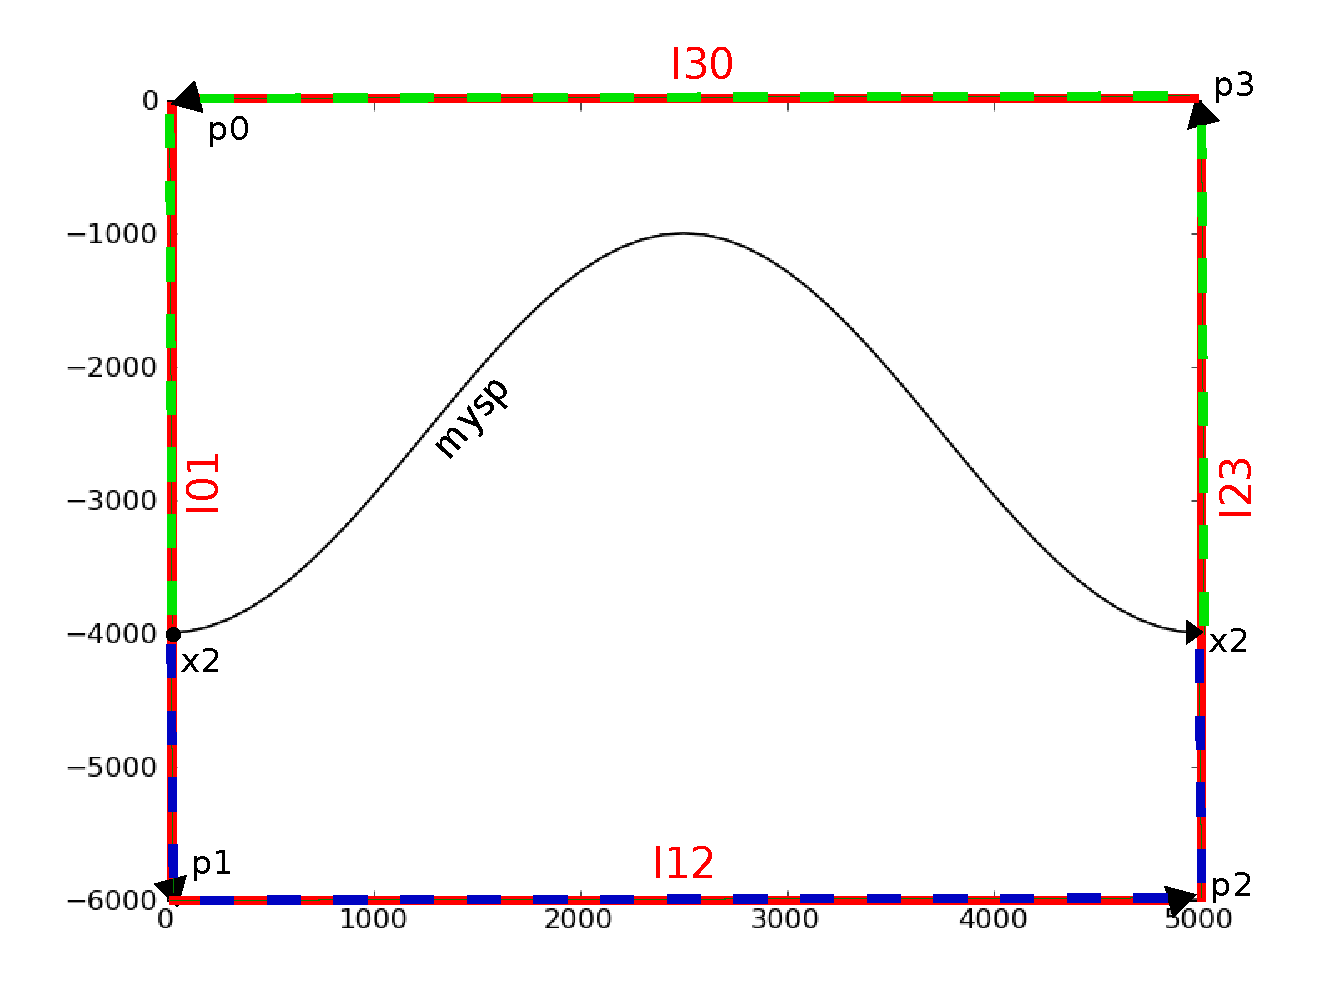
\includegraphics[width=4.in]{figures/anticlineheatrefraction}}
\caption{Heat refraction model with point and line labels.}
\label{fig:anticlinehrmodel}
\end{figure}

We will start by defining our domain and material boundaries using \pycad. This example is located in the file _________  and a labeled diagram is available in \reffig{fig:anticlinehrmodel}. As always we start with dependencies. For this example we have:
\begin{verbatim}
from esys.pycad import * #domain constructor
from esys.pycad.gmsh import Design #Finite Element meshing package
from esys.finley import MakeDomain #Converter for escript
import os #file path tool
import numpy as np #numerial python for arrays
from math import * # math package
#used to construct polygons for plotting from pycad
from cblib import getLoopCoords 
\end{verbatim}
There are two modes available in our example. When \verb modal=1  we indicate to the script that we wish to model an anticline. Othewise when \verb modal=-1  we wish to modal a syncline. The modal operator simply changes the phase of the boundary function so that it is either upwards or downwards curving. A \verb save_path  has also been defined so that we can easily separate our data from other examples and our scripts. 

It is now possible to start defining our domain and boundaries. There are a few primary constructors in \pycad that build upon each other to define domains and boundaries; the one we will use are:
\begin{verbatim}
Point() #Create a point in space.
Line() #Creates a line from a number of points.
CurveLoop() #Creates a closed loop from a number of lines.
Surface() #Creates a surface based on a CurveLoop
\end{verbatim}
We start by inputting the four corners of our domain, which from the origin has the dimensions of 5000 meters width and -6000 meters depth. This is done with the \verb Point()  function which accepts and x, y and z coordinates. Our domain is in two dimensions so z should always be zero. Be careful to define all your constructs in an \textbf{anti-clockwise} manner otherwise the meshing algorithm may fail.
\begin{verbatim}
# Overall Domain
p0=Point(0.0,        0.0, 0.0)
p1=Point(0.0,    -6000.0, 0.0)
p2=Point(5000.0, -6000.0, 0.0)
p3=Point(5000.0,     0.0, 0.0)
\end{verbatim}
Now lines are defined in an \textbf{anti-clockwise} direction using our points. This forms a rectangle around our domain.
\begin{verbatim}
l01=Line(p0, p1)
l12=Line(p1, p2)
l23=Line(p2, p3)
l30=Line(p3, p0)
\end{verbatim}
These lines form the basis for our domain boundary, which is a closed loop.
\begin{verbatim}
c=CurveLoop(l01, l12, l23, l30)
\end{verbatim}
The curve defining our clinal structure is located in approximately the middle of the domain and has a cosinusoidal shape. We define the curve by generating points at discrete intervals; 51 in this case, and then create a smooth curve through the points using the \verb Spline()  function.
\begin{verbatim}
x=[ Point(i*100.0,-2500+modal*1500.*cos(pi*i*100.0/2500.0+pi)) for i in range(0,51) ]
mysp = Spline(*tuple(x)) #*tuple() forces x to become a tuple
\end{verbatim}
The start and end points of the spline can be returned to help define the material boundaries.
\begin{verbatim}
x1=Spline.getStartPoint(mysp)
x2=Spline.getEndPoint(mysp)
\end{verbatim}
Our top block or material above the clinal/spline boundary is defined in a \textbf{anti-clockwise} manner by creating lines and then a closed loop. As we will be meshing the subdomain we also need to assign it a planar surface. 
\begin{verbatim}
# TOP BLOCK
tbl1=Line(p0,x1)
tbl2=mysp
tbl3=Line(x2,p3)
tblockloop = CurveLoop(tbl1,tbl2,tbl3,l30)
tblock = PlaneSurface(tblockloop)
\end{verbatim}
It is also necessary to create and export a polygon for \esc so that we can plot the boundaries of our subdomains. First we take the loop from our block and retreive its point coordinates with the function \verb getLoopCoords()  and then output it with \modnumpy for our solution script.
\begin{verbatim}
tpg = getLoopCoords(tblockloop)
np.savetxt(os.path.join(save_path,"toppg"),tpg,delimiter=" ")
\end{verbatim}
We must repeat the above for our every other subdomain. We have only one other, the bottom block. The process is the fairly similar to the top block but with a few differences. The spline points must be reversed by setting the spline as negative.
\begin{verbatim}
bbl4=-mysp
\end{verbatim}
This reverse spline option unfortunately does not work for the getLoopCoords command, however, the polygon tool will accept clock-wise oriented points so we can define a new curve.
\begin{verbatim}
#clockwise check
bblockloop2=CurveLoop(mysp,Line(x2,p2),Line(p2,p1),Line(p1,x1))
bpg = getLoopCoords(bblockloop2)
np.savetxt(os.path.join(save_path,"botpg"),bpg,delimiter=" ")
\end{verbatim}
The last few steps in creating our model take the previously defined domain and subdomain points and generate a mesh that can be imported into \esc.
To initial the mesh it first needs some design parameters. In this case we have 2 dimensions \verb dim  and a specified number of finite elements we wish to apply to the domain \verb element_size  . It then becomes a simlpe task of adding the subdomains and flux boundaries to the design. If we wish to give the elements names as in the example we can use the \verb PropertySet()  function. This will allow us to easily define the subdomain properties in the solution scirpt. We then save the geometry, mesh and create our \esc domain. 
\begin{verbatim}
# Create a Design which can make the mesh
d=Design(dim=2, element_size=200)
# Add the subdomains and flux boundaries.
d.addItems(PropertySet("top",tblock),PropertySet("bottom",bblock),PropertySet("linebottom",l12))
# Create the geometry, mesh and Escript domain
d.setScriptFileName(os.path.join(save_path,"heatrefraction_mesh001.geo"))
d.setMeshFileName(os.path.join(save_path,"heatrefraction_mesh001.msh"))
domain=MakeDomain(d, integrationOrder=-1, reducedIntegrationOrder=-1, optimizeLabeling=True)
# Create a file that can be read back in to python with mesh=ReadMesh(fileName)
domain.write(os.path.join(save_path,"heatrefraction_mesh001.fly"))
\end{verbatim}
The creation of our domain and its mesh is complete. Now we must create a solution for our steady state problem.


